%%%%%%%%%%%%%%%%%%%%%%%%%%%%%%%%%%%%%%%%%%%%%%%%%%%%%%%%%%%%%%%%%%%%%%%%
%% Example Slides Using the UPM Metropolis Theme
%%%%%%%%%%%%%%%%%%%%%%%%%%%%%%%%%%%%%%%%%%%%%%%%%%%%%%%%%%%%%%%%%%%%%%%%

%%%%%%%%%%%%%%%%%%%%%%%%%%%%%%%%%%%%%%%%%%%%%%%%%%%%%%%%%%%%%%%%%%%%%%%%
%% Preamble
\documentclass{beamer}
\usetheme{metropolis}
\usepackage{metropolis-upm}

%%%%%%%%%%%%%%%%%%%%%%%%%%%%%%%%%%%%%%%%%%%%%%%%%%%%%%%%%%%%%%%%%%%%%%%%
%% Data
\title{UPM Metropolis Theme}
\subtitle{Minimal Template with UPM Colors}
\author{\textbf{Ciccalè Baztán, Marco}}
\date{\today}
\institute{Universidad Politécnica de Madrid (UPM)}
\titlegraphic{\hfill
\includegraphics[height=3cm]{upm-logo.png}}

%%%%%%%%%%%%%%%%%%%%%%%%%%%%%%%%%%%%%%%%%%%%%%%%%%%%%%%%%%%%%%%%%%%%%%%%
%% Start the document
\begin{document}

%%%%%%%%%%%%%%%%%%%%%%%%%%%%%%%%%%%%%%%%%%%%%%%%%%%%%%%%%%%%%%%%%%%%%%%%
%% Title Page
\maketitle

%%%%%%%%%%%%%%%%%%%%%%%%%%%%%%%%%%%%%%%%%%%%%%%%%%%%%%%%%%%%%%%%%%%%%%%%
%% Table of Contents
\begin{frame}{Table of Contents}
  \setbeamertemplate{section in toc}[sections numbered]
  \tableofcontents
\end{frame}

\section{Introduction}

\begin{frame}{Introduction}
  Welcome to this detailed example of a presentation using the Metropolis theme.
  \begin{itemize}
    \item Minimalistic design
    \item Modern look
    \item Customizable
  \end{itemize}
\end{frame}

\section{Motivation}

\begin{frame}{Why Use Metropolis?}
  \begin{itemize}
    \item Clean and modern design
    \item Easy to customize
    \item Good defaults
    \item Active community support
  \end{itemize}
\end{frame}

\section{Content}

\begin{frame}{Figures}
  \begin{figure}
    \centering
    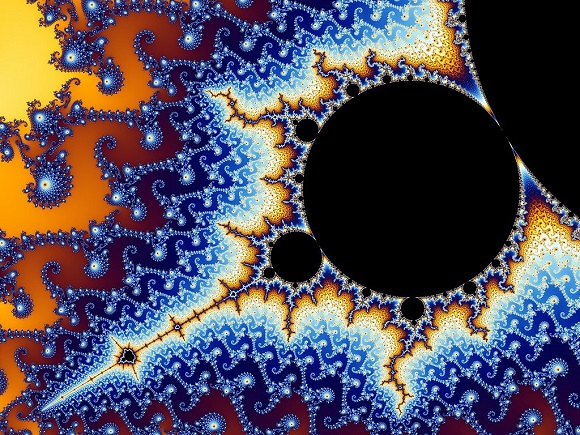
\includegraphics[width=0.5\linewidth]{fractal.jpg}
    \caption{Example Image}
  \end{figure}

\end{frame}

\begin{frame}{Tables}
  \begin{table}
    \centering
    \begin{tabular}{|c|c|c|}
      \hline
      Header 1 & Header 2 & Header 3 \\
      \hline
      Item 1 & Item 2 & Item 3 \\
      Item A & Item B & Item C \\
      \hline
    \end{tabular}
    \caption{Example Table}
  \end{table}
\end{frame}

\begin{frame}{Mathematical Content}
  The Metropolis theme supports mathematical content:
  \begin{equation}
    E = mc^2
  \end{equation}
  \begin{align}
    a^2 + b^2 &= c^2 \\
    \nabla \cdot \mathbf{E} &= \frac{\rho}{\epsilon_0}
  \end{align}
\end{frame}

\begin{frame}{Lists}
  You can use different types of lists:

  \begin{itemize}
    \item Item 1
    \item Item 2
    \item Item 3
  \end{itemize}

  \begin{enumerate}
    \item First
    \item Second
    \item Third
  \end{enumerate}

\end{frame}

\begin{frame}{Blocks}
  You can add different types of blocks:
  \metroset{block=fill}
  \begin{block}{Block Title}
    This is a block with some text.
  \end{block}
  \begin{alertblock}{Alert Block}
    This is an alert block.
  \end{alertblock}
  \begin{exampleblock}{Example Block}
    This is an example block.
  \end{exampleblock}

\end{frame}

%%%%%%%%%%%%%%%%%%%%%%%%%%%%%%%%%%%%%%%%%%%%%%%%%%%%%%%%%%%%%%%%%%%%%%%%
%% Questions
\setbeamertemplate{frame numbering}[none]
{\setbeamercolor{palette primary}{fg=white, bg=orange}
\begin{frame}[standout]
  Thank You!\\Questions?
\end{frame}
}

\end{document}

%%% Local Variables:
%%% mode: latex
%%% TeX-master: t
%%% End:
